\section{Schnyder Woods}\label{sw}
Schnyder Wälder, im weiteren \textit{Schnyder Woods}, wurden zuerst von Walter Schnyder zur Betrachung der Ordungs-Dimension planarer Graphen, als eine Färbung und Orientierung auf den inneren Kanten einer Triangulierung, betrachtet \cite{schnyder89}. In einem weiteren Resultat dienten sie zur Erlangung einer planaren Einbettung auf einem $n-2 \times n-2$ Netz\cite{schnyder90}. Im Folgenden werden wir die Verallgemeinerung auf 3-zusammenhängende plane Graphen durch Felsner \cite{felsner01} und die zu ihnen in Bijektion stehenden Schnyder Labelings einführen und uns dabei an \cite{felsner04} orientieren.\\

Für den Rest dieses Kapitels meinen wir mit $G$, wenn nicht weiter spezifiziert, einen 3-zusammenhängenden planen Graphen mit Aufhängungen $a_1,s_2,a_3$.

\begin{definition}[Schnyder Woods]
Ein Schnyder Wood ist eine Orientierung und Beschriftung der Kanten von $G$ mit den Labeln 1, 2 und 3, unter Berücksichtigung der folgenden Regeln\footnote{Alternativ wird hier auch anschaulicher von rot, grün und blau als Platzhalter für 1, 2 und 3 gesprochen. Es wird davon ausgegangen, dass die Label zyklisch sortiert sind, sodass $i+1$ und $i-1$ immer definiert sind.}:
\begin{itemize}
\item[W1] Jede Kante ist entweder un- oder bigerichtet. Falls sie bigerichtet ist haben beide Richtungen unterschiedliche Label.
\item[W2] An jeder Aufhängung  $a_i$ exisitert eine nach ausssen gerichtete Kante ohne Endpunkt mit Label i.  
\item[W3] Jeder Knoten $v$ hat hat Ausgangsgrad eins zu jedem Label. Um $v$ existieren im Uhrzeigersinn eine Auskante mit Label 1, null oder mehr eingehende Kanten mit Label 3, eine Auskante mit Label 2, null oder mehr  eingehende Kanten mit Label 1, eine Auskante mit Label 2 und null oder mehr  eingehende Kanten mit Label 2.
\item[W4] Es existiert inneres Gebiet mit gerichteten Zykel in einer Farbe als Rand.
\end{itemize}
\end{definition}

\begin{figure}[h]
	\centering
  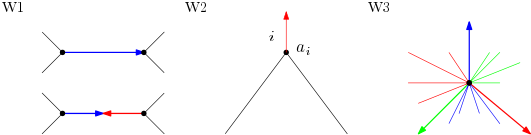
\includegraphics[width=0.8\textwidth]{schnyder_wood_def.png}
	\label{10_example}
\end{figure}

Die Existenz von Schnyder Wood für jeden 3-zusammenhängenden planen Graphen werden wir weiter unten zeigen. Zunächst wollten wir uns mit Resultaten im Bezug auf Einbettungen befassen.
Wir wollen hier kurz, das \textit{face-counting}\cite{felsner01} erläutern. Betrachten wir also $G$ zusammen mit einem Schnyder Wald $T_1,T_2,T_3$. Nach \cite[Korollar 2.5]{felsner04} handelt es sich bei den $T_i$ um gerichtete Bäume mit Wurzeln in $a_i$. Zu jedem Knoten $v$ existierten also eindeutige Pfade $P_i(v)$ zu den Aufhängungen $a_i$. Die Pfade von $v$ zu den Aufhängungen treffen sich nach \cite[Lemma 2.4]{felsner04} nur in $v$. Somit können wir zu jedem Knoten $v$ die von den Pfaden $P_{i-i}(v)$ und $P_{i+1}$ und dem äusseren Gebiet begrenzte Region $R_i$ betrachten. Durch das Zählen der Gebiete in den diesen Regionen lässt sich nun eine konvexe Zeichnung von $G$ erzeugen.

\begin{figure}[h]
	\centering
  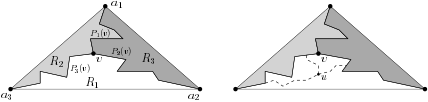
\includegraphics[width=0.8\textwidth]{schnyder_reg.png}
	\caption{Regionen zu $v$ und die Inklusion von $R_i(u)$ in $R_i(v)$ falls $u \in R_i(v)$.}
\end{figure}

Hierzu ordnet man jedem Knoten $v$ seien Gebiets Vektor $(v_1,v_2,v_3)$ zu, wobei $v_i$ die Anzahl der inneren Gebiete in $R_i$ beschreibt. Nun gilt für jeden Knoten $v_1+v_2+v_3 = |F|-1$. Seien $\alpha_1 = (0,1),\alpha_2 = (1,0)$ und $\alpha_3 = (0,0)$, dann erhalten wir die Zeichnung durch die Funktion 
$$\mu:v\to v_1\alpha_1 + v_2\alpha_2+v_3\alpha_3.$$ 
Nach \cite[Theorem 2.7]{felsner04} ist die mit diesen Koordinaten erzeugte Zeichnung planar und konvex. Sie hat sogar noch die schöne Eigenschaft, dass sich die Knoten an jedem innern Gebiet auf dem Rand eines Dreiecks befinden, wie in Abbildung \ref{schnyder_tri} illustriert.\
// TODO Schnyder Triangle Bild ?!

Eine weitere Methode um aus Schnyder Woods, über geodätische Einbettung, zu einer konvexen Zeichnung zu gelangen, wird ebenfalls in \cite{felsner04} beschrieben.

\begin{definition}[Schnyder Labeling]
Ein Schnyder Labeling ist eine Beschriftung Winkel von $G$ mit den Labeln 1, 2 und 3 unter Berücksichtigung der folgenden Regeln:
\begin{itemize}
\item[L1] Um jedes innere Gebiet bilden die Label im Uhrzeigersinn nichtleere Intervalle von 1en, 2en und 3en. Am äusseren Gebiet gilt dies gegen den Uhrzeigersinn.
\item[L2] Um jeden inneren Knoten bilden die Label im Uhrzeigersinn nichtleere Intervalle von 1en, 2en und 3en.
\item[L3] An Aufhängung $a_i$ haben äusseren Winkel die Label i-1 und i+1 im Uhrzeigersinn mit der halben Auskante dazwischen und die inneren Winkel das Label i.
\end{itemize} 
\end{definition}

\begin{figure}[h]
	\centering
  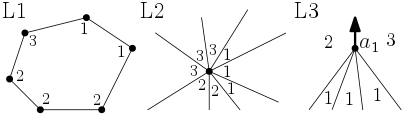
\includegraphics[width=0.8\textwidth]{schnyder_label_def.png}
	\label{10_example}
	\caption{Aus L1 und L2 folgt, dass es in einem Schnyder Labeling nur Kanten von Typ A oder B,  siehe Abbildung \ref{schnyder_bij}, gibt.}
\end{figure}

Durch Abbildung \ref{schnyder_bij} wird eine Verbindung zwischen Schnyder Woods und Schnyder Labelings geschaffen. Wenn wir uns auf drei-zusammenhängende planare Graphen beschränken, dann ist die dargestellte Abbildung nach \cite[Theorem 2.3]{felsner04} eine Bijektion.

\begin{figure}[h]
	\centering
  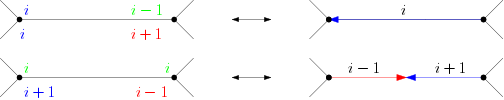
\includegraphics[width=0.9\textwidth]{schnyder_bij.png}
	\label{schnyder_bij}
	\caption{}
\end{figure}

Mithilfe der Schnyder Labelings können wir kurz auf die Existenz einer Schnyder Woods, bzw. Schnyder Labelings, für einen beliebigen 3-zusammenhängenden planen Graphen eingehen. Der 

